\begin{frame}{My Research}
\begin{itemize}
    \item \small {\textit{Polyanya} only work for single pair shortest path}
    \item My research:
        \begin{itemize}
            \item \small{multi-targets search based on framework of \textit{Polyanya}}
            \item \small{with good scalability}
        \end{itemize}
\end{itemize}
\end{frame}

\begin{frame}[fragile]{Proposed algorithm 1: brute-force \textit{Polyanya}}
\small{A naive solution is calling \textit{Polyanya} for each target:}
\onslide<2->
\begin{lstlisting}[language=python]
for t in targets:
  polyanya.run(q, t)
\end{lstlisting}
\begin{itemize}
    \item<3->\small{Drawback: inefficient when targets many.}
\end{itemize}
\end{frame}

\begin{frame}{Proposed algorithm 2: interval heuristic}
\begin{minipage}{.6\textwidth}
\begin{itemize}
\item \small {Let's review the evaluation function in \textit{Polyanya}}
\item \small {When there are multiple targets...}
\begin{itemize}
    \item \small {\textit{h-value} shouldn't affected by a specific target}
\end{itemize}
\item \small {How about remove $t$ from \textit{h-value}}?
\end{itemize}
\end{minipage}%
\begin{minipage}{.4\textwidth}
    \begin{adjustbox}{max totalsize={.9\textwidth}{.9\textheight}, right}
    \begin{tikzpicture}
        \coordinate (a) at (2, 5);
\coordinate (b) at (5, 2);
\coordinate (r) at (2, 3);
\coordinate (t1) at (5, 4);
\coordinate (t2) at (2, 6);
\coordinate (t3) at (3, 2);
\coordinate (q) at (1, 1);

\newcommand{\nodelabel}[2] {
    \node[fill,circle,scale=0.2,label=#2:$#1$,color=red] at (#1) {$#1$};
}

\newcommand{\drawST}[2] {
    \node[fill,circle,scale=0.2,label=#2:$#1$,color=blue] at (#1) {$#1$};
}

\newcommand{\snode}{
    \draw [gray] (a)--(b);
    \drawST{q}{right}
    \drawST{t1}{above}
    \nodelabel{r}{below}
    \nodelabel{a}{above}
    \nodelabel{b}{above}
}

\newcommand{\gvalue}{
    \draw [->,black, very thick] (q.north) to [out=30,in=150] (r.north);
}

\newcommand{\hvalue}{
    \draw[black,dashed,very thick] (r)--(t1);
}
        \onslide<1->{
            \snode
            \gvalue
            \hvalue
        }
        \onslide<2->{
            \drawST{t2}{above}
            \drawST{t3}{below}
        }
    \end{tikzpicture}
    \end{adjustbox}
\end{minipage}
\end{frame}

\begin{frame}{Proposed algorithm 2: interval heuristic}
\begin{minipage}{.5\textwidth}
Then we get: Interval heuristic
\begin{itemize}
    \item \textit{g-value} is same
    \item \textit{h-value}: distance from $r$ to $I$
\end{itemize}
\end{minipage}%
\begin{minipage}{.4\textwidth}
    \begin{adjustbox}{max totalsize={.9\textwidth}{.9\textheight}, right}
    \begin{tikzpicture}
        \coordinate (a) at (2, 5);
\coordinate (b) at (5, 2);
\coordinate (r) at (2, 3);
\coordinate (t1) at (5, 4);
\coordinate (t2) at (2, 6);
\coordinate (t3) at (3, 2);
\coordinate (q) at (1, 1);

\newcommand{\nodelabel}[2] {
    \node[fill,circle,scale=0.2,label=#2:$#1$,color=red] at (#1) {$#1$};
}

\newcommand{\drawST}[2] {
    \node[fill,circle,scale=0.2,label=#2:$#1$,color=blue] at (#1) {$#1$};
}

\newcommand{\snode}{
    \draw [gray] (a)--(b);
    \drawST{q}{right}
    \drawST{t1}{above}
    \nodelabel{r}{below}
    \nodelabel{a}{above}
    \nodelabel{b}{above}
}

\newcommand{\gvalue}{
    \draw [->,black, very thick] (q.north) to [out=30,in=150] (r.north);
}

\newcommand{\hvalue}{
    \draw[black,dashed,very thick] (r)--(t1);
}
        \hivalue
    \end{tikzpicture}
    \end{adjustbox}
\end{minipage}
\end{frame}

\begin{frame}{Interval heuristic: drawback}
\begin{minipage}{.4\textwidth}
\begin{itemize}
    \item<2-> \small{
        \textit{interval heuristic} causes redundant expansions
    }
    \item<3-> \small{
        especially in sparse targets scenario
    }
    \item<4-> \small{
        e.g.: query is "nearest storage locations where capacity $>=100$".
    }
    \item<5-> \small{we need a smarter evaluation function...}
\end{itemize}
\end{minipage}%
\begin{minipage}{.6\textwidth}
    \begin{adjustbox}{max totalsize={.9\textwidth}{\textheight}, right}
    \begin{tikzpicture}
        \newcommand{\nodelabel}[2] {
    \fill[red] (#1) circle[radius=.5ex];
    \node[#2] at (#1) {#1};
}

\newcommand{\medge}[2]{
    \draw[gray,thick] (#1)--(#2);
}

\newcommand{\drawVs}{
    %\nodelabel{a}{above}
    \nodelabel{b}{below}
    \nodelabel{c}{below}
    
    %\nodelabel{d}{left}
    \nodelabel{e}{right}
    \nodelabel{f}{below}
    
    \nodelabel{g}{above}
    \nodelabel{h}{below}
    %\nodelabel{i}{below}
}

\newcommand{\drawmeshs}{
    \medge{a}{k},\medge{a}{d},\medge{a}{b},\medge{a}{c}
    \medge{b}{c},
    \medge{c}{g}
    \medge{d}{f},\medge{d}{l},\medge{d}{e}
    \medge{l}{f}
    \medge{e}{c},\medge{e}{f}
    \medge{f}{h}
    \medge{g}{h},\medge{g}{b}
    \medge{h}{i}
}

\newcommand{\drawobstacles}{
    \fill[black] (a)--(b)--(c)--cycle;
    \fill[black] (g)--(h)--(i)--cycle;
    \fill[black] (d)--(e)--(f)--cycle;
}

%\coordinate (a) at (2, 6); 
\coordinate (a) at (0, 7);
\coordinate (b) at (8, 7); 
\coordinate (c) at (6, 5); 
\coordinate (d) at (1, 3);
\coordinate (e) at (4, 3);
\coordinate (f) at (4, 2);
\coordinate (g) at (7, 4);
\coordinate (h) at (7, 2);
%\coordinate (i) at (9, 0);
\coordinate (i) at (10, 0);
\coordinate (j) at (5, 2);
\coordinate (k) at (0, 7);
\coordinate (l) at (0, 0);
\coordinate (m) at (10, 0);
\coordinate (n) at (10, 7);
\coordinate (q) at (3, 4);
\coordinate (t) at (9, 3); 
% boundary
\draw[black, ultra thick] (k)--(n)--(m)--(l)--cycle;

% obstacles
\drawobstacles
% mesh
\drawmeshs
% vertices
\drawVs
% start
\fill[blue] (q) circle[radius=.5ex];
\node[above] at (q) {$q$};
% end
\fill[blue] (t) circle[radius=.5ex];
\node[above] at (t) {$t$};
        \intervalexpansion
    \end{tikzpicture}
    \end{adjustbox}
\end{minipage}
\end{frame}


\begin{frame}{Proposed algorithm 3: target heuristic}
\begin{minipage}{.5\textwidth}
\small{Let me introduce the detail of \textit{h-value} in \textit{Polyanya},\\
$h_p(node, t)$ equals}:
\begin{itemize}
    \item \small Case 1: $d_e(r, t_1)$
    \item \small Case 2: $d_e(r, a) + d_e(a, t_2)$
    \item \small Case 3: when $r$ and $t_3$ at same side, compute mirror point of $t_3$, and go to Case 1 or Case 2
    
\end{itemize}

\end{minipage}%
\begin{minipage}{.5\textwidth}
    \begin{adjustbox}{max totalsize={.9\textwidth}{.9\textheight}, right}
    \centering
    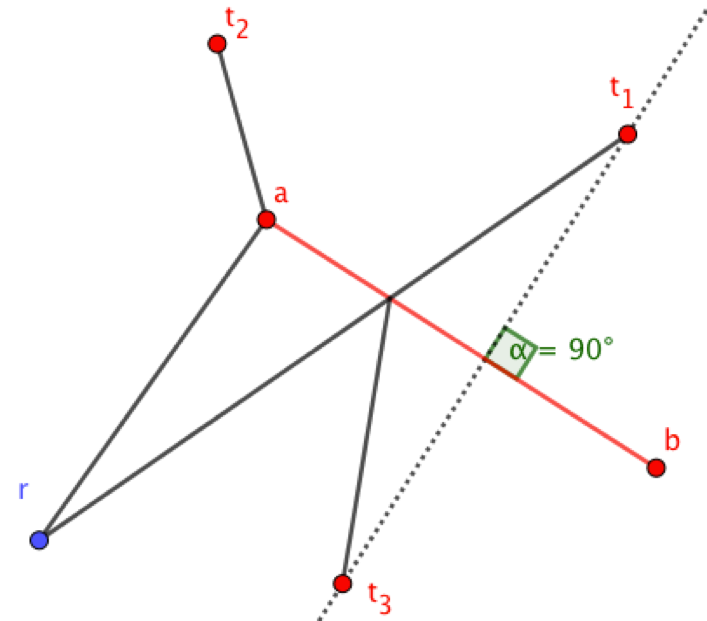
\includegraphics{pic/ef.png}
    \end{adjustbox}
\end{minipage}
\end{frame}

\begin{frame}{Proposed algorithm 3: target heuristic}
\setbeamercovered{invisible}
\small{
When there are multiple targets ...
}
\onslide<2->{
    \begin{definition}{closest target of search node}
    is a target $t$ that $h_p(node, t)$ is minimal.
    \end{definition}
}
\onslide<3->
\small{
    How to find the closest target for a search node?
}
\end{frame}

\begin{frame}{Proposed algorithm 3: target heuristic}
  \begin{itemize}
    \item \small {In Case 3, instead of flipping targets, we can flip the $r$}
    \item \small{
Let $NN_e(\textit{area, p})$: traditional nearest neighbor of \textit{p} in \textit{area}.
    }
  \end{itemize}

\begin{minipage}{.35\textwidth}
  \begin{itemize}
    \item \only<3-> {$\scriptstyle NN_e(\scriptscriptstyle{areaA \cup areaA'}, \scriptstyle a)$ \small or}
    \item \only<4-> {$\scriptstyle NN_e(\scriptscriptstyle{areaB \cup areaB'}, \scriptstyle b)$ \small or}
    \item \only<5-> {$\scriptstyle NN_e(areaC, r)$ \small or}
    \item \only<6-> {$\scriptstyle NN_e(areaC', r')$}
    \item \only<7-> {\small Choose the best}
  \end{itemize}
\end{minipage}%
\begin{minipage}{.6\textwidth}
    \begin{adjustbox}{max totalsize={\textwidth}{\textheight}, right}
        \begin{tikzpicture}[line cap=round,line join=round,>=triangle 45,x=2.0cm,y=2.0cm]
        \definecolor{zzwwqq}{rgb}{0.6,0.4,0.}
\definecolor{ccqqqq}{rgb}{0.8,0.,0.}
\definecolor{qqwwtt}{rgb}{0.,0.4,0.2}
\definecolor{ududff}{rgb}{0.30196078431372547,0.30196078431372547,1.}
\coordinate (a) at (2.5, 2.5);
\coordinate (b) at (3.5, 2.5);
\coordinate (c) at (3.2, 2.5);
\coordinate (r) at (3, 2);
\coordinate (r') at (3, 3);
\coordinate (t1) at (1.63, 2.28);
\coordinate (t2) at (1.33, 3);
\coordinate (t3) at (2.5, 3);
\coordinate (t4) at (3.5, 3.5);
\coordinate (t5) at (4.18, 2.82);
\coordinate (t6) at (4.52, 2.27);
\coordinate (t7) at (3.5, 1.7);
\coordinate (t8) at (2.5, 1.5);

\newcommand{\nodelabel}[2] {
    \node[fill,circle,scale=0.25,label=#2:$#1$,color=ududff] at (#1) {$#1$};
}

%\draw [line width=2.pt,dash pattern=on 2pt off 2pt,domain=-0.7621281650478093:3.0] plot(\x,{(-2.5--0.5*\x)/-0.5});
%\draw [line width=2.pt,dash pattern=on 2pt off 2pt,domain=3.0:5.571634219160852] plot(\x,{(-0.5--0.5*\x)/0.5});
%\draw [line width=2.pt,dash pattern=on 2pt off 2pt,domain=-0.7621281650478093:3.0] plot(\x,{(-0.-0.5*\x)/-0.5});
%\draw [line width=2.pt,dash pattern=on 2pt off 2pt,domain=3.0:5.571634219160852] plot(\x,{(--3.-0.5*\x)/0.5});

\newcommand{\drawra}{
  \draw [line width=1.pt,dash pattern=on 1pt off 3pt,domain=1.0:3.0] plot(\x,{(-2.5--0.5*\x)/-0.5});
}
\newcommand{\drawrb}{
  \draw [line width=1.pt,dash pattern=on 1pt off 3pt,domain=3.0:5.0] plot(\x,{(-0.5--0.5*\x)/0.5});
}
\newcommand{\drawrpa}{
  \draw [line width=1.pt,dash pattern=on 1pt off 3pt,domain=1.0:3.0] plot(\x,{(-0.-0.5*\x)/-0.5});
}
\newcommand{\drawrpb}{
  \draw [line width=1.pt,dash pattern=on 1pt off 3pt,domain=3.0:5.0] plot(\x,{(--3.-0.5*\x)/0.5});
}

\newcommand{\areaA}{
  \fill[line width=2.pt,color=ccqqqq,fill=ccqqqq,fill opacity=0.1] (2.5,2.5) -- (1.,4.) -- (1.,2.5) -- cycle;
  \draw[color=ccqqqq] (1.24, 3.3) node {$areaA$};
}

\newcommand{\areaAp}{
  \fill[line width=2.pt,color=ccqqqq,fill=ccqqqq,fill opacity=0.1] (1.,2.5) -- (1.,1.) -- (2.5,2.5) -- cycle;
  \draw[color=ccqqqq] (1.25, 2) node {$areaA'$};
  \draw [line width=1.pt,dash pattern=on 1pt off 3pt,domain=1.0:3.0] plot(\x,{(-2.5--0.5*\x)/-0.5});
}

\newcommand{\areaB}{
  \fill[line width=2.pt,color=zzwwqq,fill=zzwwqq,fill opacity=0.1] (3.5,2.5) -- (5.,4.) -- (5.,2.5) -- cycle;
  \draw[color=zzwwqq] (4.6,3.28) node {$areaB$};
  \draw [line width=1.pt,dash pattern=on 1pt off 3pt,domain=3.0:5.0] plot(\x,{(-0.5--0.5*\x)/0.5});
}

\newcommand{\areaBp}{
  \fill[line width=2.pt,color=zzwwqq,fill=zzwwqq,fill opacity=0.1] (5.,2.5) -- (3.5,2.5) -- (5.,1.) -- cycle;
  \draw[color=zzwwqq] (4.5,2.) node {$areaB'$};
}
\newcommand{\areaC}{
  \fill[line width=2.pt,color=qqwwtt,fill=qqwwtt,fill opacity=0.25] (1.,4.) -- (5.,4.) -- (3.5,2.5) -- (2.5,2.5) -- cycle;
  \draw[color=qqwwtt] (2.768699664953716,3.536745981551138) node {$areaC$};
}

\newcommand{\areaCp}{
  \fill[line width=2.pt,color=qqwwtt,fill=qqwwtt,fill opacity=0.25] (2.5,2.5) -- (3.5,2.5) -- (5.,1.) -- (1.,1.) -- cycle;
  \draw[color=qqwwtt] (2.9078624650952896,1.2962248992718015) node {$areaC'$};
}

\newcommand{\dashh}{
  \draw [line width=1.pt,dash pattern=on 1pt off 3pt,domain=1.:5.] plot(\x,{(--2.5-0.*\x)/1.});
}

\newcommand{\caseA}{
  \draw [red, dashed] (t2)--(a);
  \draw [red] (t1)--(a);
  \nodelabel{t1}{left}
  \nodelabel{t2}{left}
}

\newcommand{\caseB}{
  \draw [red, dashed] (t6)--(b);
  \draw [red] (t5)--(b);
  \nodelabel{t5}{right}
  \nodelabel{t6}{right}
}

\newcommand{\caseC}{
  \draw [red, dashed] (t4)--(r);
  \draw [red] (t3)--(r);
  \nodelabel{t3}{left}
  \nodelabel{t4}{right}
}

\newcommand{\caseCp}{
  \draw [red, dashed] (t8)--(r');
  \draw [red] (t7)--(r');
  \nodelabel{t8}{left}
  \nodelabel{t7}{right}
}

\newcommand{\drawbg}{
  \clip(1.,1.) rectangle (5.,4.);
  \dashh
  \draw[gray, line width=2pt] (a)--(b);
  \nodelabel{a}{above}
  \nodelabel{b}{below}
  \nodelabel{r}{below}
  \nodelabel{r'}{above}
}

\newcommand{\drawbest}{
  \areaA
  \areaAp
  \areaB
  \areaBp
  \areaC
  \areaCp
  \drawra
  \drawrb
  \drawrpa
  \drawrpb
  \draw[red, dashed] (t1)--(a);
  \draw[red, dashed] (a)--(r);
  \draw[red, dashed] (t5)--(b);
  \draw[red, dashed] (b)--(r);
  \draw[red, dashed] (r)--(c);
  \draw[red, dashed] (c)--(t7);
  \draw[red] (r)--(t3);


  \nodelabel{t1}{left}
  \nodelabel{t5}{right}
  \nodelabel{t3}{left}
  \nodelabel{t7}{right}
}

          \only<2-> \drawbg
          \uncover<3> \areaA
          \uncover<3> \areaAp
          \only<3> \drawra
          \only<3> \drawrpa
          \only<3> \caseA
          \uncover<4> \areaB
          \uncover<4> \areaBp
          \only<4> \drawrb
          \only<4> \drawrpb
          \only<4> \caseB
          \uncover<5> \areaC
          \only<5> \drawra
          \only<5> \drawrb
          \only<5> \caseC
          \uncover<6> \areaCp
          \only<6> \drawrpa
          \only<6> \drawrpb
          \only<6> \caseCp
          \only<7> \drawbest
        \end{tikzpicture}
    \end{adjustbox}
\end{minipage}
\end{frame}

\begin{frame}{Proposed algorithm 3: target heuristic}
\begin{minipage}{.9\textwidth}
\begin{itemize}
    \onslide<1-> \item \small{
        For each successor, assign the closest target to it
    }
    \onslide<2-> \item \small {
    Correctness:
    \begin{lemma}{Non-decreasing property:}
        Whenever the closest target of a search node changes,
        the \textit{h-value} never decrease.
    \end{lemma}
    }
\end{itemize}
\end{minipage}%
\end{frame}

\begin{frame}{Proposed algorithm 3: target heuristic}
\setbeamercovered{invisible}
\begin{minipage}{.9\textwidth}
\begin{itemize}
    \item \small{Four \textit{R-tree} queries for each search  node is expensive}
    \item \small{So we are looking for further refinements...}
\end{itemize}
\end{minipage}%
\end{frame}

\begin{frame}{Proposed algorithm 3: target heuristic refinements}
\setbeamercovered{invisible}
\begin{minipage}{.9\textwidth}
\begin{itemize}
    \item \small{Lazy query}
    \begin{Definition}
        In expansion, instead of finding a new target, successors can inherit the closest target from their parent if the \textit{h-value} doesn't change.
    \end{Definition}
    \item \small{Correctness}
    \begin{lemma}
        In this case, it is impossible to find a target with less \textit{h-value}.
    \end{lemma}
\end{itemize}
\end{minipage}%
\end{frame}

\begin{frame}{Proposed algorithm 3: target heuristic refinements}
\setbeamercovered{invisible}
\begin{minipage}{.9\textwidth}
\begin{itemize}
    \item \small{Reassignment}
    \begin{definition}
        \small Once $t$ be retrieved, we must reassign another target to those search nodes who are regarding $t$ as their closest target
    \end{definition}
    \item \small{Lazy reassignment}
    \begin{definition}
        \small Instead of exploring the entire open list, we can do reassignment when such search node pop out
    \end{definition}
    \item \small{Correctness}
    \begin{lemma}
        \small Lazy reassignment doesn't change relative expansion order.
    \end{lemma}
\end{itemize}
\end{minipage}%
\end{frame}
